\chapter{EXPERIMENTS}

\textbf{Experimental setup:} We evaluated the proposed improvements – fixed cross-entropy loss, ranking max loss functions $&$ adding additional samples – on four dataset. RSC15 is based on the dataset of RecSys Challange 2015\footnote[9]{http://2015.recsyschallenge.com}, which contains click and buy events from an online webshop. We only kept the click data. VIDEO and VIDXL are proprietary datasets containing watch events from an
online video service. Finally, CLASS is a proprietary dataset containing item page view events from an online classified site. Datasets were subjugated to minor preprocessing then split into train and test sets so that a whole session either belongs to the train or to the test set. The split is based on the time of the first event of the sessions. The datsets and the split are exactly the same for RSC15 as \cite{hidasi2016a}; and for VIDXL and CLASS as in \cite{hidasi2015session}. VIDEO is of the same source as in \cite{hidasi2016a}, but a slightly different subset. Table~\ref{table1}  overviews the main properties of the datasets.


% Please add the following required packages to your document preamble:
% \usepackage{multirow}

\begin{table}[htbp]
\centering
\caption{Properties of the datasets.} 
\label{table1} 


\begin{tabular}{llllll}
\hline
\multicolumn{1}{c}{\multirow{}{}{\textbf{Data}}} & \multicolumn{2}{c}{\textbf{Train set}} & \multicolumn{2}{c}{\textbf{Test set}} & \multicolumn{1}{c}{\multirow{}{}{\textbf{Items}}} \\
\multicolumn{1}{c}{}                               & \multicolumn{2}{c}{Sessions}           & \multicolumn{2}{c}{Sessions}          & \multicolumn{1}{c}{}                                \\
\hline
RSC15                                              & 7.999.257          & 31.637.239        & 15.324            & 71.222            & 37.483                                              \\
VIDEO                                              & 2.144.930          & 10.214.429        & 29.804            & 153.157           & 262.05                                              \\
VIDXL                                              & 17.419.964         & 69.312.698        & 216.725           & 921.202           & 712.824                                             \\
CLASS                                              & 1.173.094          & 9.011.321         & 35.745            & 254.857           & 339.055                                            
\end{tabular}
\end{table}

Evaluation is done under the next item prediction scenario, that is we iterate over test sessions and events therein. For each event, the algorithm guesses the item of the next event of that session. Since the size of the VIDXL test set is large, we compare the target item’s score to that of the 50,000 most popular items during testing, similarly to \cite{hidasi2016a}. While this evaluation for VIDXL overestimates the performance, the comparison of algorithms remain fair \cite{bellogin2011precision}. As recommender systems can only recommend a few items at once, the actual item a user might pick should be amongst the first few items of the list. Therefore, our primary evaluation metric is recall@20 that is the proportion of cases having the desired item amongst the top-20 items in all test cases. Recall does not consider the actual rank of the item as long as it is amongst the top-N. This models certain practical scenarios well where there is no highlighting of recommendations and the absolute order does not matter. Recall also usually correlates well with important online KPIs, such as click-through rate (CTR)\cite{liu2012enlister}; \cite{hidasi2012fast}. The second metric used in the experiments is MRR@20 (Mean Reciprocal Rank). That is the average of reciprocal ranks of the desired items. The reciprocal rank is set to zero if the rank is above 20. MRR takes into account the rank of the item, which is important in cases where the order of recommendations matter (e.g. the
lower ranked items are only visible after scrolling).

The natural baseline we use is the original GRU4Rec algorithm, upon which we aim to improve. We consider the results with the originally proposed TOP1 loss and tanh activation function on the
output to be the baseline. The hidden layer has 100 units. We also indicate the performance of item-kNN, a natural baseline for next item prediction. Results for RSC15, VIDXL and CLASS are
taken directly from corresponding papers \cite{hidasi2016a};b and measured with the optimal hyperparameters in \cite{hidasi2016a} for VIDEO. We do separate hyperparameter optimization on a separate validation set for the proposed improvements.

The methods are implemented under the Theano framework 
\cite{al2016theano}in python. Experiments were run on various GPUs, training times were measured on an unloaded Titan X (Maxwell) GPU. Code is available publicly on GitHub \footnote[10]{https://github.com/blinded} for reproducibility.

\subsection{USING ADDITIONAL SAMPLES}
The first set of experiments examines the effect of additional negative samples on recommendation
accuracy. Experiments were performed on the CLASS and the VIDEO datasets. Since results are quite similar we excluded the VIDEO results to save some space. Figure \ref{fig:fig2}a depicts the performance of the network with TOP1, cross-entropy, TOP1-max and BPR-max losses. Recommendation accuracy was measured with different number of additional samples, as well as in the case when all scores are computed and there is no sampling. As we discussed earlier, this latter scenario is a more theoretical one, because it is not scalable. As theory suggests (see Section \ref{sec:loss}), the TOP1 loss does not cope well with lots of samples. There is a slight increase in performance with a few extra samples, as the chance of having relevant samples increases; but performance quickly degrades as sample size grow, thus lots of irrelevant samples are included. On the other hand, all three of the other losses react well to adding more samples. The point of diminishing return is around a few thousand of extra samples for cross-entropy. TOP1-max starts to slightly lose accuracy after that. BPR-max improves with more samples all the way, but slightly loses accuracy when all items are used.

\begin{figure}[htp]
    \centering
    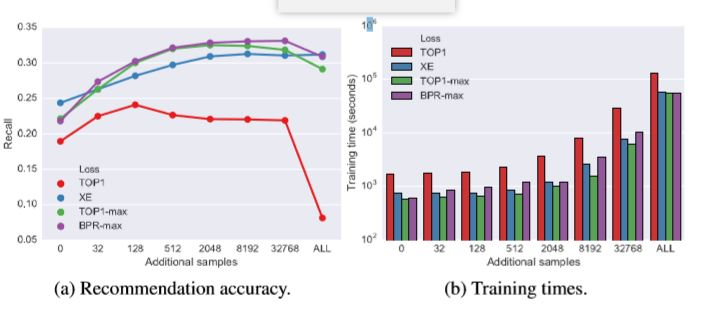
\includegraphics[width=400]{img/p3.JPG}
    \caption{Results on the CLASS dataset. ”ALL” means no sampling of items.}
    \label{fig:fig3}
\end{figure}

Adding extra samples increase computational cost, yet due to easy parallelization on modern GPUs most of this cost is alleviated. Figure \ref{fig:fig2} shows the training times at different sample sizes. Please note the logarithmic scale. The actual training time depends on not just the dataset, but model parameters (especially mini-batch size) and how certain operators used for computing the loss are supported by the framework. The trend, however, is similar to for all losses. For example, the full training of the network is around 10 minutes (with the settings for cross-entropy or TOP1-max), which does not increase with even 512 extra samples. At the point of diminishing returns, i.e. at 2048 extra samples, training time is around 15 minutes, which is also totally acceptable. After that, training times grow quickly, due to exceeding the parallelization capabilities of the GPU we used. The trend is similar on the VIDEO dataset, with training times starting around 50 minutes,starting to increase at 2048 extra samples (to 80 minutes) and quickly above thereafter. This means that the proposed method can be used with zero too little additional cost in practice, unlike data augmentation methods. It is also clear that GRU4Rec can work just as well with a few thousands of negative examples as with the whole itemset, thus it can be kept scalable.

In the next experiment we perform a parameter sensitivity analysis of the α parameter that controls the sampling. Figure \ref{fig:fig4} depicts the performance over different α values for the cross-entropy, TOP1- max and BPR-max losses. Cross-entropy favors higher α values with low sample sizes and low $\alpha$
values for large samples. This is inline with our discussion in Section \ref{sec:sample}: popular samples are useful
when the sample size is very limited and at the beginning of the training, but might be exhausted
quickly, thus switching to a more balanced sampling can be beneficial if we have the means to (e.g.
large enough sample size). Also, the uniform sampling in this case is supplemented by the few


\begin{figure}[htp]
    \centering
    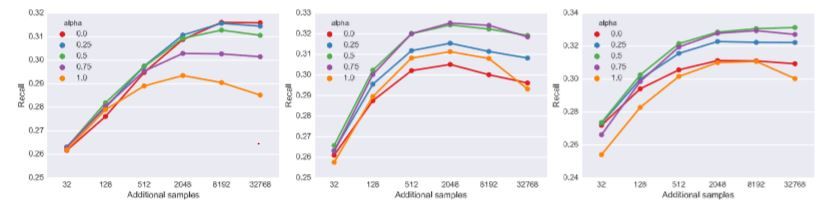
\includegraphics[width=400]{img/p4.JPG}
    \caption{The effect of the alpha parameter on recommendation accuracy at different sample sizes
on the CLASS dataset. Left: cross-entropy loss; Middle: TOP1-max loss; Right: BPR-max loss.}
    \label{fig:fig4}
\end{figure}

popularity based samples of the mini-batch sampling. The ranking-max losses, on the other hand, seem to prefer the middle road with a slight preference towards higher values, while the extremes perform the worst. We assume that this is mostly due to (a) being based on pairwise losses, where popular samples are usually desired; (b) and the score regularization: with popularity based sampling the scores of the most popular items would be decreased beyond what is desirable.

Table 2: Recommendation accuracy with additional samples and different loss functions compared to item-kNN and the original GRU4Rec. Improvements over item-kNN and the original GRU4Rec (with TOP1 loss) results are shown in parentheses. Best results are typeset bold.


\begin{table}[htbp]
  \centering
  \caption{Marks of Students}
    \begin{tabular}{|r|l|r|r|}
		\hline
    S. No. &Name& Roll No. &Marks \\
		\hline
    1     & Arshad & 1234  & 80 \\
    2     & Hamid & 1235  & 75 \\
    3     & Shariq & 1236  & 82 \\
    4     & Ahmed & 1237  & 68 \\
    5     & Asif  & 1238  & 74 \\
		\hline
		\hline
    \end{tabular}%
  \label{tab:addlabel}%
\end{table}%

\label{headings}


\subsection{LOSS - FUNCTIONS}

We measure the performance gain of the proposed improvements over the baselines. The big accuracy improvement comes from the combination of additional samples and the loss functions (fixed cross-entropy, TOP1-max and BPR-max). Table 2 showcases our most important results. Besides the original version of GRU4Rec and the item-kNN, we included results with cross-entropy (XE) loss without additional sampling to confirm that the fixed cross-entropy loss still performs just slightly better than TOP1. The increase with sampling and the proper loss function is stunning as the best results exceed the accuracy of the original GRU4Rec by 15 − 35\% and that of item-kNN by up to 52\%. BPR-max even performs slightly better (+1 − 7\%) than cross-entropy on 3 of 4 datasets and achieves similar results on the remaining one dataset.

On \cite{tan2016improved} reported $∼ 0.685$ and $∼ 0.29$ in recall@20 and MRR@20 respectively \footnote[11]{Read from figure4. Unfortunately, the results in table1 are for networks trained on various subsets of the
training set.} using data augmentation. Unlike our solutions, data augmentation greatly increases training
times. Data augmentation and our improvements are not mutually exclusive, thus it is possible that
combining the two methods, even better results can be achieved. A very recent paper \cite{chatzis2017recurrent} proposes the Bayesian version of GRU4Rec and reports $\sim $ 0.61 and $\sim $ 0.25 in recall@20 and MRR@20 when using 100 units \footnote[12]{Based on figure1. Their best results (0.6507 and 0.3527) are achieved using 1500 units, which is highly impractical. Even though, our version still performs better wrt. recall when compared to this much bigger network.} . Therefore our GRU4Rec version is the current best performer so far.


\begin{table}[htbp]
\label{table:table3}
  \centering
  \caption{Marks of Students}
    \begin{tabular}{|r|l|r|r|}
		\hline
    S. No. &Name& Roll No. &Marks \\
		\hline
    1     & Arshad & 1234  & 80 \\
    2     & Hamid & 1235  & 75 \\
    3     & Shariq & 1236  & 82 \\
    4     & Ahmed & 1237  & 68 \\
    5     & Asif  & 1238  & 74 \\
		\hline
		\hline
    \end{tabular}%
  \label{tab:addlabel}%
\end{table}%


\subsection{UNIFIED ITEM REPRESENTATIONS}
Previous experiments did not find any benefits of using an embedding layer before the GRU layers. The role of the embedding layer is to translate item IDs into the latent representation space. In the recommender systems terminology, item embeddings correspond to “item feature vectors”. The network has another “item feature matrix” in the form of the output weight matrix. By unifying the representations, i.e. sharing the weight matrix between the embedding layer and the output layer, we learn better item representations quicker. Preliminary experiments (Table \ref{table:table3}) show additional improvements in recall@20 and slight decrease in MRR@20 for most of the datasets, however, for the CLASS dataset both recall and MRR are increased significantly when unified embeddings are used (+15.02\% and +21.87\% in recall and MRR respectively, compared to the model trained
without embeddings).



\label{headings}


\section{CONCLUSION}
We introduced a new class of loss function that together with an improved sampling strategy have provided impressive top-k gains for RNNs for session-based recommendations. We believe that these new losses could be more generally applicable and along with the corresponding sampling strategies also provide top-k gains for different recommendations settings and algorithms such as e.g. matrix factorization or auto encoders. It is also conceivable that these techniques could also provide similar benefits in the area of Natural Language Processing a domain that shares significant similarities to the recommendation domain in terms of machine learning (e.g. ranking, retrieval) and data structure (e.g. sparse large input and output space).

